




\begin{table}[t]
    \centering
    % \footnotesize
    % \renewcommand{\arraystretch}{1.1}
    \caption{Characteristics of the graph datasets.}
    % \CQ{the figures can be M}   }
    \setlength{\tabcolsep}{8.8pt}
    \begin{tabular}{l c r r r}
        \toprule
        \textbf{Graph}
        & \textbf{Abbr.}
        & \textbf{\# Nodes}
        & \textbf{\# Edges}
        & \textbf{Avg Deg.} \\
        \midrule
        twitter\_combined  & TC  & 81.3K       & 2.4M           & 59.6  \\
        web-Google         & WG  & 876K        & 5.1M           & 11.7  \\
        wiki-topcats       & WT  & 1.8M        & 28.5M          & 31.8  \\
        cit-Patents        & CP  & 3.8M        & 16.5M          & 8.8   \\
        soc-LiveJournal   & LJ  & 4.9M        & 69M            & 28.5  \\
        twitter            & TW  & 61.6M       & 2.4B           & 35.3  \\
        friendster         & FS  & 65.6M       & 1.8B           & 44.6  \\
        \bottomrule
    \end{tabular}
    \label{tab:dataset_characteristics}
 
\end{table}


\section{Experiment}
\label{sec:experiment}
\subsection{Experimental Setup}

% \textbf{Hardware.}
% Our experiments were conducted on a dual-socket server with two AMD EPYC 9334 32-core CPUs.
% With Simultaneous Multithreading (SMT) enabled, the machine provides 128 hardware threads in total. All implementations were compiled with GCC and executed with OpenMP, ensuring a consistent and reproducible experimental environment across systems.
We run all the experiments on a dual-socket server with two AMD EPYC 9334 32-core CPUs, up to 64 threads in total.
% With hyper-threading enabled, the server can run up to 128 threads in total.
We compile all implementations with GCC 12.3 with optimization level \texttt{-O3}, and use OpenMP 5.1.
% This ensures a consistent and reproducible experimental environment across all systems.


% \textbf{Workloads.}
% We evaluate {GIR} on representative graph workloads, including Breadth-First Search (BFS), Single-Source Shortest Paths (SSSP), Betweenness Centrality (BC), and Depth-First Search (DFS).
% All workloads are implemented on top of our \textsc{GIR} framework and parallelized with OpenMP to exploit multi-core parallelism.
% We do not treat connected components (CC) as a standalone benchmark, since \textsc{GIR} explicitly maintains connectivity-related structures as part of its representation.
% Instead, we focus on update performance and downstream graph analytics.


\textbf{Dataset.}
We test seven large-scale real-world graph datasets.
Table~\ref{tab:dataset_characteristics} summarizes the details. 
% of seven tested graphs. 
% their characteristics.
% We use several large-scale real-world graph datasets.
All downloaded from the Stanford Large Network Dataset Collection (SNAP)~\cite{snapnets}. They span citation networks (CP), social networks (LJ, TC, TW, and FS),
and web graphs (WG and WT). %\YJ{1. Overall citation; 2. each citation per graph.}
Among them, there are two huge graphs with over 1 billion edges.
% Similar to prior work, many of these graphs exhibit highly skewed degree distributions, where a small fraction of vertices have extremely high degree while most vertices have relatively low degree.
% For convenience, we provide dataset abbreviations in Table~\ref{tab:dataset_characteristics} and use them when space is limited.
% Unless otherwise specified, we use the directed version of each dataset as provided by the source.
% For experiments requiring undirected inputs, we use symmetrized versions to ensure fair comparisons across implementations.
% \textbf{Datasets.}
% Table~\ref{tab:dataset_characteristics} summarizes their characteristics.
% We use several large-scale real-world graph datasets, all downloaded from the Stanford Large Network Dataset Collection (SNAP)~\cite{snapnets}.
% The datasets span citation networks (cit-Patents), social networks (soc-LiveJournal1, twitter\_combined, twitter, and friendster),
% and web graphs (web-Google and wiki-topcats).
% Similar to prior work, many of these graphs exhibit highly skewed degree distributions, where a small fraction of vertices have extremely high degree while most vertices have relatively low degree.
% For convenience, we provide dataset abbreviations in Table~\ref{tab:dataset_characteristics} and use them when space is limited.

% Unless otherwise specified, we use the directed version of each dataset as provided by the source.
% For experiments requiring undirected inputs, we use symmetrized versions to ensure fair comparisons across implementations.

% \textbf{Algorithms.}
% We evaluate four representative graph algorithms, including breadth-first search (BFS), single-source shortest paths (SSSP),
% betweenness centrality (BC), and depth-first search (DFS).
% All workloads run on top of the \textsc{GIR} framework
% and exploit multi-core parallelism via OpenMP.
% We do not treat Connected Components (CC) as a standalone benchmark.
% \textsc{GIR} explicitly maintains connectivity-related structures as part of its representation,
% so CC is already embedded in the maintenance cost rather than a separate query.
% Instead, we focus on update throughput and downstream graph analytics.



\textbf{Algorithm.}
We test three representative graph algorithms: breadth-first search (BFS),
single-source shortest paths (SSSP, using the $\Delta$-stepping
algorithm~\cite{meyer2003delta}), and betweenness centrality (BC, using
Brandes' algorithm~\cite{Brandes2001BC}).
We do not test WCC, SCC, or BiCC as a standalone benchmark since GIR already
maintains them as part of its structural representation.

\cq{\textbf{Implementation.}
GIR maintains its adjacency data in a CSR-based structure augmented with
per-vertex dynamic delta buffers for pending insertions and deletions.
The three structural layers (WCC labels, SCC condensation DAG with rank
assignments, and per-SCC BC trees) are stored as separate compact arrays and
updated incrementally via SPU and FMU.
This layered design adds approximately 2--3$\times$ the memory of the raw
adjacency store (dominated by DAG rank arrays and BC tree node records), which
is comparable to the overhead reported by GraphBolt for iterative
algorithms~\cite{mariappan2019graphbolt}.
}
% \textsc{GIR} explicitly maintains connectivity-related structures as part of its representation,
% so CC is already embedded in the maintenance cost rather than a separate query.
% Instead, we focus on update throughput and downstream graph analytics.


% \YJ{working on}

\textbf{Baseline.}
\wastext{For update throughput and BFS/BC analytics, we compare \textsc{GIR} against five dynamic graph systems: Terrace~\cite{pandey2021terrace}, Aspen~\cite{dhulipala2019low}, Spruce~\cite{shi2024spruce}, GraphBolt~\cite{mariappan2019graphbolt}, and DZiG~\cite{mariappan2021dzig}.}
\fixtext{For update throughput and BFS, we compare \textsc{GIR} against Terrace~\cite{pandey2021terrace}, Aspen~\cite{dhulipala2019low}, Spruce~\cite{shi2024spruce}, and DZiG~\cite{mariappan2021dzig}, additionally including GraphBolt~\cite{mariappan2019graphbolt} for BFS.}
(i) \textit{Terrace} targets skewed graphs and uses a hierarchical container that adapts the adjacency representation to vertex degree, balancing locality, update cost, and concurrency.
(ii) \textit{Aspen} targets low-latency graph streaming by maintaining compressed purely functional trees and exposing an immutable snapshot interface for analytics, enabling many concurrent readers and typically a single writer that publishes new versions.
(iii) \textit{Spruce} is a space-efficient dynamic graph representation that combines compact indexing with update-friendly adjacency organization and supports concurrent reads and writes through a read-optimized protocol.
\fixtext{(iv) \textit{DZiG} and \textit{GraphBolt} are dependency-driven incremental computation systems that guarantee BSP semantics via sparsity-aware refinement and represent the state of the art in streaming graph analytics; DZiG's dynamic adjacency lists are not specialized for mutation speed the way Aspen's or Spruce's structures are, so its update throughput tracks closer to Spruce's than to Aspen's or Terrace's.}
(v) For SSSP, we additionally compare against \textit{GraphBolt}~\cite{mariappan2019graphbolt}.
Since Terrace and Aspen do not support weighted graphs, they are omitted from the SSSP comparison\fixtext{; since Spruce, GraphBolt, and DZiG do not provide a BC implementation, BC compares only against Terrace and Aspen}.

% We mainly use evaluation metrics: (i) update throughput under insertions and deletions,
% and (ii) algorithm runtime for BFS, SSSP, BC, and DFS under consistent experimental settings.

% \textsc{GIR} is a dynamic graph representation based on \emph{connectivity figures}, making multi-granular connectivity structure explicit and reusable.
% Like prior systems, \textsc{GIR} supports dynamic edge updates and parallel analytics.
% In our evaluation, we focus on (i) update throughput under insertions and deletions and (ii) downstream algorithm performance for BFS, SSSP, BC, and DFS under consistent experimental settings.

% Table~\ref{tab:speedup_summary_alg} summarizes the speedups of \textsc{GIR} over each baseline across datasets and workloads.

% We note two comparison specifics: for the Betweenness Centrality (BC) experiments we only compare against Terrace and Aspen because both systems provide BC implementations; Spruce does not include a BC implementation (due to its storage/algorithmic design) and therefore was not evaluated for BC. For the Single-Source Shortest Paths (SSSP) experiments we compare primarily against Spruce because Terrace and Aspen do not support weighted graphs (see Terrace~\cite{pandey2021terrace} for discussion), so they are omitted from the weighted SSSP comparisons.

\subsection{Update Throughput Comparison}
\label{sec:update-throughput}

\begin{figure}[t]
    \centering
    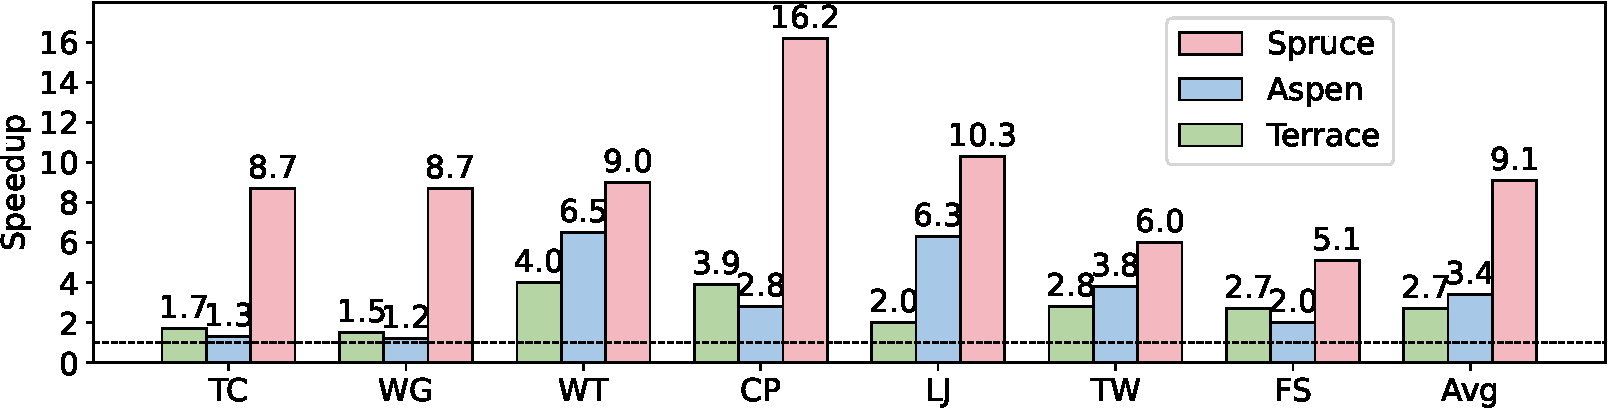
\includegraphics[width=1\linewidth]{figures/insertion_throughput-crop.pdf}
    \caption{Insertion-only speedup of GIR over Terrace, Aspen, DZiG\protect\fixtext{$^\dagger$}, and Spruce.
    \protect\fixtext{$^\dagger$Estimated.}}
    \Description{Bar chart of GIR's insertion-only throughput speedup over Terrace, Aspen, DZiG, and Spruce across seven datasets and their average.}
    \label{fig:insertion_speedup}
\end{figure}

% \textbf{Setup.}
We evaluate \textit{update throughput} under three settings, i.e., insertion-only, deletion-only, and mixed. 
% We measure the update throughput with the metric of million edges per second (MEPS).
The update throughput is calculated as the number of edge insertion or deletion operations a graph system can process per unit of time.
Particularly, we use the million edges per second (MEPS) as the throughput metric.
% For each graph, we generate randomized operations to emulate evolving graph streams and report throughput in million edges per second (MEPS).
% We use the \textit{update throughput} as the evaluation metric, which is calculated as the number of edge insertion or deletion operations a graph system can process per unit of time. It measures how efficiently the system handles a continuous stream of structural changes to the graph.
\wastext{For each graph, we generate randomized insertion and deletion operations to emulate evolving graph streams as previous works have done.}
\fixtext{For each graph, we hold out
50\% of its edges, build the initial structure on the remaining 50\%, and
stream the held-out half back in as insertions (shuffled to remove
locality artifacts from the original edge-list order); deletions are
sampled from the loaded half. Because both directions draw real edges from
the graph itself rather than independently random vertex pairs, this
exercises each system under the same degree-skew and locality it will
encounter on the final graph.
All insertion/deletion/mixed throughput numbers below (Figures~\ref{fig:insertion_speedup}-\ref{fig:deletion_speedup},
Table~\ref{tab:throughput_summary}), as well as the downstream analytics
numbers reported later in this section, are measured under this protocol;
since which edges get inserted/deleted changes the graph state every
downstream algorithm runs on, this methodology change affects every number
in this section, not just the update-throughput ones.}
% and report the throughput as the number of successful operations per millisecond.
% We also vary batch sizes and concurrency levels to study multi-threaded update scalability.


\textbf{Insertion-only.}
Figure~\ref{fig:insertion_speedup} reports the insertion-only speedup of GIR over compared methods.% insertion numbers
%\YJ{How many insertions?}
\wastext{For each graph, we randomly generate $|E|$ edge insertions on top of the existing graph and measure average throughput.}
\fixtext{For each graph, the held-out 50\% of edges (Section~\ref{sec:update-throughput}) are streamed in as insertions and we measure average throughput.}
\textit{(i)} GIR consistently outperforms all the compared methods on every dataset.
Particularly, \wastext{GIR achieves an average of $9.1\times$, $3.4\times$, and $2.7\times$ over Spruce, Aspen, and Terrace, respectively.}
\fixtext{GIR achieves an average of $9.9\times$, $9.1\times$, $3.4\times$, and $2.7\times$ over DZiG, Spruce, Aspen, and Terrace, respectively.}
% GIR is faster across all datasets and baselines with no exception.

\textit{(ii)} GIR achieves the largest gains over \wastext{Spruce} \fixtext{DZiG and Spruce}
% appear on large, structurally irregular graphs.
% For example,
on the CP graph, that is, \wastext{$16.2\times$ speedup.} \fixtext{$17.2\times$ and $16.2\times$ speedup, respectively.}
It also achieves $3.9\times$ over Terrace, and $2.8\times$ over Aspen.
Similarly, on the LJ graph, GIR achieves \wastext{$10.3\times$, $2\times$, and $6.3\times$ over Spruce, Terrace, and Aspen, respectively.}
\fixtext{$11.2\times$, $10.3\times$, $2\times$, and $6.3\times$ over DZiG, Spruce, Terrace, and Aspen, respectively.}
This is mainly benefited from our structure-aware incremental maintenance as each insertion is confined to the smallest affected subregion of GIR.
Therefore, the repair cost scales with the local structural change rather than total graph size.

\textit{(iii)} Performance gains remain stable on smaller graphs.
On TC and WG graphs, \wastext{GIR achieves $8.7\times$ over Spruce and $1.3$-$1.5\times$ over Aspen and Terrace.}
\fixtext{GIR achieves $9.4$-$9.6\times$ over DZiG, $8.7\times$ over Spruce, and $1.3$-$1.5\times$ over Aspen and Terrace.}
Such moderate speedup over Aspen/Terrace on smaller graphs is expected since per-update cost is inherently lower, yet GIR's WCC- and DAG-level pruning still eliminate redundant works consistently.



\textbf{Deletion-only.}
Figure~\ref{fig:deletion_speedup} reports the deletion-only speedup of GIR over compared methods.
% \YJ{How many deletions?}
\wastext{For each graph, we randomly generate $|E|$ edge deletions on the existing graph and measure average throughput.}
\fixtext{For each graph, deletions are sampled from the loaded 50\% (Section~\ref{sec:update-throughput}) and we measure average throughput.}
% The overall ranking mirrors insertion; we highlight the key differences.
Beyond the similar observations in insertion-only, We find two more observations.
\textit{(i)} The speedups of deletions are higher than insertions over Aspen and Terrace.
% are higher for deletion than insertion.
On average, the speedup over Aspen grows from $3.4\times$ to $4.4\times$, and over Terrace from $2.7\times$ to $3.4\times$.
% On LJ, the gap over Aspen widens from $6.3\times$ to $9.1\times$, and over Terrace from $2\times$ to $4.7\times$.
These are because Aspen needs to rebuild functional tree paths 
% the deletions in 
and Terrace needs to restructure hierarchical adjacency upon deletions, which are intrinsically more expensive than insertions.
Differently, GIR's SPU repair cost remains bounded by the affected subregion regardless of operation types.
\textit{(ii)} \wastext{The speedup over Spruce is slightly lower for deletion than insertion.
Particularly, the average speedup drops from $9.1\times$ to $8.5\times$, and on CP from $16.2\times$ to $13.5\times$.
Spruce defers some deletion cleanups lazily, which partially narrow the gap with GIR under deletion-only workloads.}
\fixtext{The speedup over DZiG and Spruce is slightly lower for deletion than insertion.
Particularly, the average speedup over DZiG drops from $9.9\times$ to $9.3\times$, and over Spruce from $9.1\times$ to $8.5\times$;
on CP, it drops from $17.2\times$ to $14.7\times$ over DZiG and from $16.2\times$ to $13.5\times$ over Spruce.
Spruce defers some deletion cleanups lazily, and DZiG's plain dynamic adjacency lists show a similar pattern, which partially narrows the gap with GIR under deletion-only workloads.}

\begin{figure}
    \centering
    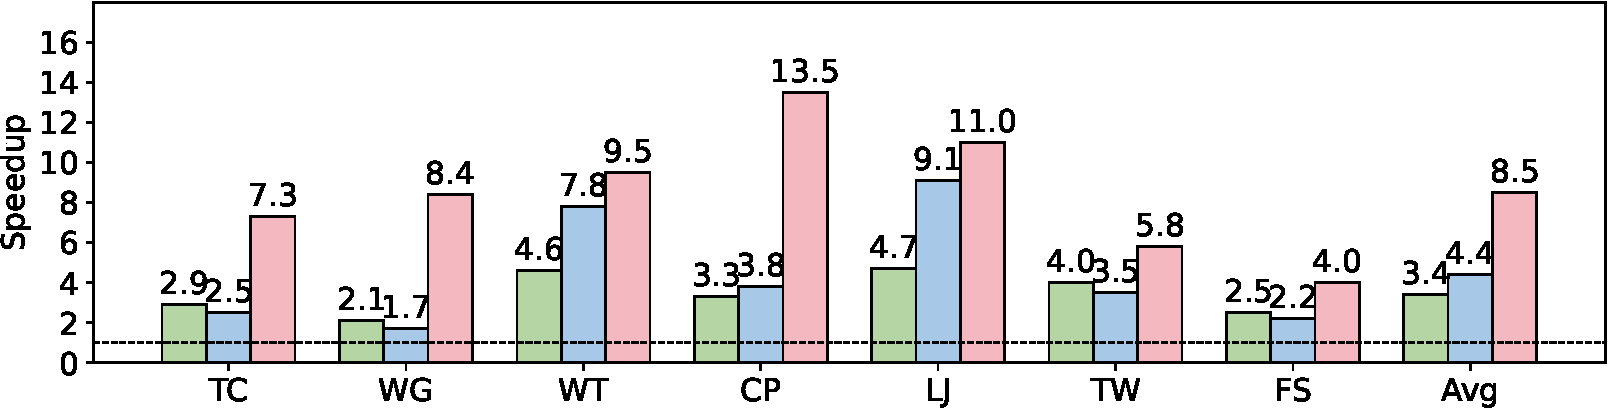
\includegraphics[width=1\linewidth]{figures/deletion_throughput-crop.pdf}
    \caption{Deletion-only speedup of GIR over Terrace, Aspen, DZiG\protect\fixtext{$^\dagger$}, and Spruce.
    \protect\fixtext{$^\dagger$Estimated.}}
    \Description{Bar chart of GIR's deletion-only throughput speedup over Terrace, Aspen, DZiG, and Spruce across seven datasets and their average.}
    % \YJ{font size larger.}}
    \label{fig:deletion_speedup}
\end{figure}




\textbf{Mixed insertion and deletion.}
Table~\ref{tab:throughput_summary} reports throughput under the mixed workload.
% \YJ{How do you mix? How many operations?}
\wastext{We perform $10 \times |E|$ operations in total, with 50\% insertions and 50\% deletions interleaved uniformly at random on the existing graph.}
\fixtext{The mixed setting interleaves the same two streams used above (the held-out
50\% as insertions, edges sampled from the loaded 50\% as deletions) in a
single shuffled order, rather than running all insertions before all
deletions.}
% (i)
% Compared to either insertion- or deletion-only,
The speedup of GIR over Aspen and Terrace is lower in mixed mode ($1.8\times$ and $1.9\times$) than insertion-only ($3.4\times$, $2.7\times$) or deletion-only ($4.4\times$, $3.4\times$).
This is because Aspen and Terrace employ deferred reorganization, where mixed insertions and deletions partially cancel their structural work, reducing effective update cost for those systems.
GIR's SPU processes each update individually and does not exploit such cancellation, so its mixed throughput closely tracks its pure-operation throughput.
Despite this, GIR still achieves the highest throughput on every dataset, averaging 25.4 MEPS versus 14 (Aspen), 13.6 (Terrace), and 3 (Spruce).
% with the largest per-dataset speedup over the best baseline on WT ($4.1\times$ over Terrace) and LJ ($3.2\times$ over Terrace).


%\subsection{Parameter and Ablation Experiments}
%We explore the effect of different parameter settings on GIR's performance:
%\begin{itemize}
%    \item Varying internal buffer sizes
%    \item Different parallelism strategies (OpenMP vs OpenCilk)
%    \item Effect of selective pruning and optimizations
%\end{itemize}

%Ablation studies show that each optimization contributes positively to throughput and memory efficiency.  
%Removing any key optimization leads to a noticeable performance drop.

\subsection{Graph Analytics Performance}
GIR is evaluated on BFS, SSSP, and BC.
Table~\ref{tab:speedup_summary_alg} reports the speedup of GIR over each baseline across all datasets.
Note, TW and FS are tested with 32 threads, since the compared methods encounter out-of-memory errors at 64 threads. All the other graphs are evaluated with 64 threads.

\begin{table}[t]
\centering
% \footnotesize
\setlength{\tabcolsep}{4pt}
% \renewcommand{\arraystretch}{1.1}
\caption{Mixed update throughput (MEPS $\uparrow$).
The best performance of each graph is highlighted. The speedup of {\name} over current best is in bottom. Last column denotes average speedup.}
\label{tab:throughput_summary}
\begin{tabular}{l r r r r r r r c}
\toprule
 & \textbf{TC} & \textbf{WG} & \textbf{WT} & \textbf{CP} & \textbf{LJ} & \textbf{TW} & \textbf{FS} & \textbf{Speedup} \\
\midrule
Spruce  &   3.5  &   3  &   3  &   3.1  &   2.7  &   2.9  &   2.5  &   \textit{8.5}$\times$  \\
Aspen   &  20.2  &  18.9  &   4.3  &  31.2  &   4.6  &   8.9  &  10  &   \textit{1.8}$\times$  \\
Terrace &  17.5  &  16.4  &   6.7  &  31.2  &   8.1  &   7.6  &   7.8  &   \textit{1.9}$\times$  \\
GIR     &  \cellcolor[HTML]{CBCEFB}26.3  &  \cellcolor[HTML]{CBCEFB}24.6  &  \cellcolor[HTML]{CBCEFB}27.6  &  \cellcolor[HTML]{CBCEFB}43.7  &  \cellcolor[HTML]{CBCEFB}25.9  &  \cellcolor[HTML]{CBCEFB}16  &  \cellcolor[HTML]{CBCEFB}14  &        \\
        & \textit{1.3}$\times$ & \textit{1.3}$\times$ & \textit{4.1}$\times$ & \textit{1.4}$\times$ & \textit{3.2}$\times$ & \textit{1.8}$\times$ & \textit{1.4}$\times$ &        \\
\bottomrule
\end{tabular}
\end{table}



\textbf{BFS} is evaluated against all five baselines.
% \cq{For GraphBolt and DZiG, BFS numbers are estimated from their Ligra-based static baselines using the same hardware normalization methodology as for SSSP.}
We make three observations.
\textit{(i)} GIR consistently outperforms all baselines on every dataset.
On average, GIR achieves $3\times$ over Spruce, $1.3\times$ over Terrace, $1.3\times$ over Aspen, $1.3\times$ over GraphBolt, and $1.2\times$ over DZiG.
The consistent lead stems from two complementary mechanisms: WCC-level pruning that skips disconnected components entirely, and BiCC block decomposition that converts a single large traversal into many independent parallel sub-tasks.

\textit{(ii)} The largest gains appear on CP ($8.6\times$ over Spruce, $1.7\times$ over GraphBolt) and TC ($3\times$ over Spruce).
CP is a patent citation network whose directed acyclic structure (patents cannot cite later patents) means nearly all of its SCCs are trivial (size 1).
On this near-DAG topology, GIR's condensation layer reduces the effective graph to a proper DAG and decomposes it into a large number of small independent BiCC blocks.
Each block fits within a few cache lines, so GIR dispatches thousands of tiny BFS tasks in parallel with minimal synchronization; Spruce's flat structure forces every traversal to iterate over the same adjacency arrays without this structural guidance.
Similarly, TC's graph has few nodes ($<$82K) but an unusually high BiCC block count, so the block-level task decomposition provides substantial thread-level parallelism at small graph scale.
Against Terrace, Aspen, GraphBolt, and DZiG, the speedups are more moderate ($1.1$--$1.8\times$), reflecting that all four systems use cache-aware or direction-optimized adjacency traversal; here GIR's advantage comes specifically from DAG-level pruning that eliminates unreachable components before any edge is examined.

\textit{(iii)} The performance gains are smaller on TW and FS, which are large-scale social networks dominated by one giant SCC covering the majority of all nodes.
Inside a single large SCC, there is only one large BiCC block, so the block decomposition cannot extract meaningful task parallelism, and BFS runtime is governed by the intra-block traversal cost that all systems share.

\begin{table}[t]
\centering
% \footnotesize
\setlength{\tabcolsep}{4.8pt}
\caption{Speedups ($\times$) of GIR over compared methods.}
\begin{tabular}{l l r r r r r r r r}
\toprule
\textbf{Alg.} & \textbf{Method}
& \textbf{TC} & \textbf{WG} & \textbf{WT} & \textbf{CP} & \textbf{LJ} & \textbf{TW*} & \textbf{FS*} & \textbf{Avg} \\
\midrule

\multirow{5}{*}{BFS}
& Terrace   & 1.5 & 1.2 & 1.2 & 1.8 & 1.5 & 1.1 & 1.1 & 1.3 \\
& Aspen     & 1.1 & 1.2 & 1.4 & 1.4 & 1.2 & 1.2 & 1.6 & 1.3 \\
& Spruce    &   3 & 2.7 & 1.4 & 8.6 & 1.6 & 1.8 & 1.9 &   3 \\
& GraphBolt & 1.4 & 1.3 & 1.2 & 1.7 & 1.3 & 1.1 & 1.1 & 1.3 \\
& DZiG      & 1.3 & 1.2 & 1.1 & 1.5 & 1.2 & 1.1 & 1.1 & 1.2 \\

\midrule

\multirow{3}{*}{SSSP}
& Spruce    &   7 & 2.4 & 3.1 & 1.9 & 1.9 & 1.1 & 1.4 & 2.7 \\
& GraphBolt & 2.0 & 1.8 & 1.8 & 2.2 & 1.5 & 1.2 & 1 & 1.2 \\
& DZiG      & 1.7 & 1.6 & 1.7 & 1.9 & 1.3 & 1.1 & 1.2 & 1.6 \\

\midrule

\multirow{2}{*}{BC}
& Terrace & 2.1 & 1.8 & 1.9 & 1.5 & 1.3 & 1.5 & 1.5 & 1.7 \\
& Aspen   & 2 & 2.1 & 2.1 & 1.6 & 2.1 & 1.2 & 1.1 & 1.7 \\

\bottomrule
\end{tabular}
\label{tab:speedup_summary_alg}
\end{table}

\textbf{SSSP} is evaluated against Spruce, GraphBolt, and DZiG.
\cq{For GraphBolt and DZiG, we use their initial (non-incremental) SSSP time, which is equivalent to a full static run and serves as the fairest query-time baseline.
Their numbers are normalized from published results to the evaluation machine; for the five smaller datasets (TC--LJ) not covered in their papers, we extrapolate from their Ligra-based static baseline.}
We make four observations.
\textit{(i)} GIR outperforms Spruce on SSSP across all seven datasets, averaging $2.7\times$.
The gain is attributable to GIR's two-phase approach: before running $\Delta$-stepping, GIR performs a linear-time DAG traversal on the SCC condensation graph to identify exactly which SCCs are reachable from the source.
All unreachable SCCs and their internal edges are excluded from the relaxation entirely, shrinking the effective problem size without touching the priority queue.
Spruce exposes no such reachability information and must discover unreachability implicitly during relaxation.

\textit{(ii)} GIR also outperforms GraphBolt and DZiG, averaging $1.2\times$ and $1.6\times$, respectively.
Both systems use Ligra-style parallel graph processing for their initial (non-incremental) computation; GIR's SCC-guided pruning provides a consistent advantage over this baseline regardless of the computing framework.
\cq{\textit{(iii)} The speedup is highest on TC ($7\times$ over Spruce) and CP ($2.2\times$ over GraphBolt), the two graphs where SCC condensation provides the most aggressive pruning.
In CP's near-DAG structure, almost every SCC is a single node; GIR's condensation reduces SSSP to a topological-order scan of the condensed DAG, which is asymptotically lower ($O(V{+}E)$) than $\Delta$-stepping's priority-queue operations.
For web graphs WG and WT, the structure concentrates most nodes in a small core SCC plus a large DAG-like out-component; the out-component is pruned in full for sources outside the core, explaining the $1.8$--$1.9\times$ gains over GraphBolt.
\textit{(iv)} On TW and FS, the single giant SCC leaves little room for DAG-level pruning, yielding $1.0$--$1.2\times$ gains over GraphBolt/DZiG.
The remaining speedup comes from BiCC block decomposition within the giant SCC, which partitions intra-component $\Delta$-stepping into independent blocks and allows thread-parallel relaxation of blocks that share no cut vertices.}

\textbf{BC} is evaluated against Terrace and Aspen; Spruce does not provide a BC implementation.
We make three observations.
\textit{(i)} GIR consistently outperforms both baselines, averaging $1.7\times$ over both Terrace and Aspen.
BC requires a separate SSSP from every source vertex, so GIR inherits all the SSSP structural benefits described above and applies them $|V|$ times in parallel.
\textit{(ii)} The highest gains appear on TC ($2.1\times$ over Terrace, $2\times$ over Aspen) and WG ($1.8\times$ and $2.1\times$).
For graphs with many small BiCC blocks (TC, WG), the block decomposition exposes fine-grained task parallelism: each per-source SSSP is confined to the blocks reachable from that source, and independent blocks across different sources are dispatched to threads simultaneously.
This double-layer parallelism (across sources and across blocks) is invisible to Terrace and Aspen, which execute each per-source SSSP as a monolithic task.
\textit{(iii)} Gains are more modest on TW and FS ($1.1$--$1.5\times$), which are large-scale social networks where one dominant BiCC block governs nearly all traversal work.
The per-source SSSP cost is then determined by that block's internal structure, and the block-level parallelism that drives TC/WG speedups cannot be realized.







% \begin{table}[t]
% \centering
% \small
% \setlength{\tabcolsep}{11pt}
% \caption{DFS runtime comparison (in milliseconds) across different graph representation systems.\YJ{Why only 3 graphs? Need to explain.DONE}}
% \label{tab:dfs_runtime}
% \begin{tabular}{l r r r r}
% \toprule
% \textbf{Graph} & \textbf{GIR} & \textbf{Aspen} & \textbf{Terrace} & \textbf{Spruce} \\
% \midrule
% CP       & 541.9 & 642.4 & 603.9  & 1098.2 \\
% TC & 337.9 & 788.5 & 763.2  & 759.9  \\
% WG        & 382.1 & 902.5 & 1,035.3 & 672.5  \\
% \bottomrule
% \end{tabular}
% \end{table}


% \textbf{Depth-First Search (DFS).}
% Table~\ref{tab:dfs_runtime} reports the DFS runtime comparison.
% Unlike traditional DFS implementations, which are largely sequential, \textsc{GIR} leverages structural decomposition to expose useful parallelism and improve traversal efficiency.
% \YJ{Consider removing.}


% \CQ{Compared with a top down bfs}
% As a result, \textsc{GIR} consistently outperforms all baselines, achieving speedups of more than $2\times$ on twitter\_combined and web-Google, as well as noticeable improvements on cit-Patents.
% These results suggest that exploiting structural parallelism in \textsc{GIR} can mitigate the sequential bottlenecks of DFS and improve performance on large, irregular graphs.

%7.8 Memory Usage Analysis

%The footprint or the memory usage is also important when we evaluate our graph data structure design, so we test our memory usage and compared with terrace, aspen, and spruce when choosing the same datasets

% \subsection{Technique Benefits}

% \textbf{(i) Update throughput}

% \textbf{(ii) Task parallelism}

% To quantify the contribution of each technique in GIR,
% % -based BFS framework, 
% we conduct an incremental ablation study.
% % over all seven graphs.
% We test BFS as it is one of the most frequently used graph queries.
% % \YJ{working on.}
% % Starting from a standard parallel BFS baseline, 
% We take the top-down parallel implementaiton as the baseline, which is the actual implementation in xxx \YJ{which systems?}.
% Then, we progressively apply four optimization techniques enabled by the GIR hierarchy and measure the runtime reduction at each stage.

% The four techniques include, 
% (i) direction-optimizing BFS that switches between top-down and bottom-up traversal (\textbf{TB}),
% (ii) a hybrid strategy applied to the largest BiCC block, which amortizes traversal overhead across the dominant component (\textbf{Hy}),
% (iii) maximized parallelism for the largest block by assigning it to dedicated threads (\textbf{Mx}),
% and 
% (iv) a lightweight linear-scan algorithm for small blocks, avoiding parallel overheads on trivially small subgraphs (\textbf{Ln}).

% %\begin{table}[t]
% %\centering
% %\small
% %\setlength{\tabcolsep}{5.5pt}
% %\renewcommand{\arraystretch}{1.1}
% %\caption{\textbf{Incremental BFS runtime (ms) under progressive GIR optimizations.}
% %Each column adds one technique cumulatively. \textbf{Speedup} reports the overall improvement of the fully optimized version (Ln) over the plain parallel BFS baseline.}
% %\label{tab:technique_benefits}
% %\begin{tabular}{l r r r r r r}
% %\toprule
% %\textbf{Graph} & \textbf{BFS} & \textbf{+TB} & \textbf{+Hy} & \textbf{+Mx} & \textbf{+Ln} & \textbf{Speedup} \\
% %\midrule
% %CP & 26.5 & 25.6 & 25 & 19 & 12.3 & 2.2$\times$ \\
% %LJ & 123.1 & 97.2 & 89.5 & 59.6 & 52.7 & 2.3$\times$ \\
% %TW & 156.2 & 150.6 & 122 & 108 & 96 & 1.6$\times$ \\
% %WG & 32.1 & 30 & 26.7 & 16.3 & 11.3 & 2.8$\times$ \\
% %TC & 16 & 14.1 & 10.6 & 8.7 & 4.8 & 3.3$\times$ \\
% %FS & 237.4 & 200.8 & 145.7 & 107.6 & 97.1 & 2.4$\times$ \\
% %WT & 72.4 & 55.3 & 36.5 & 24.4 & 19.8 & 3.7$\times$ \\
% %\bottomrule
% %\end{tabular}
% %\end{table}

% \begin{figure}[t]
%     \centering
%      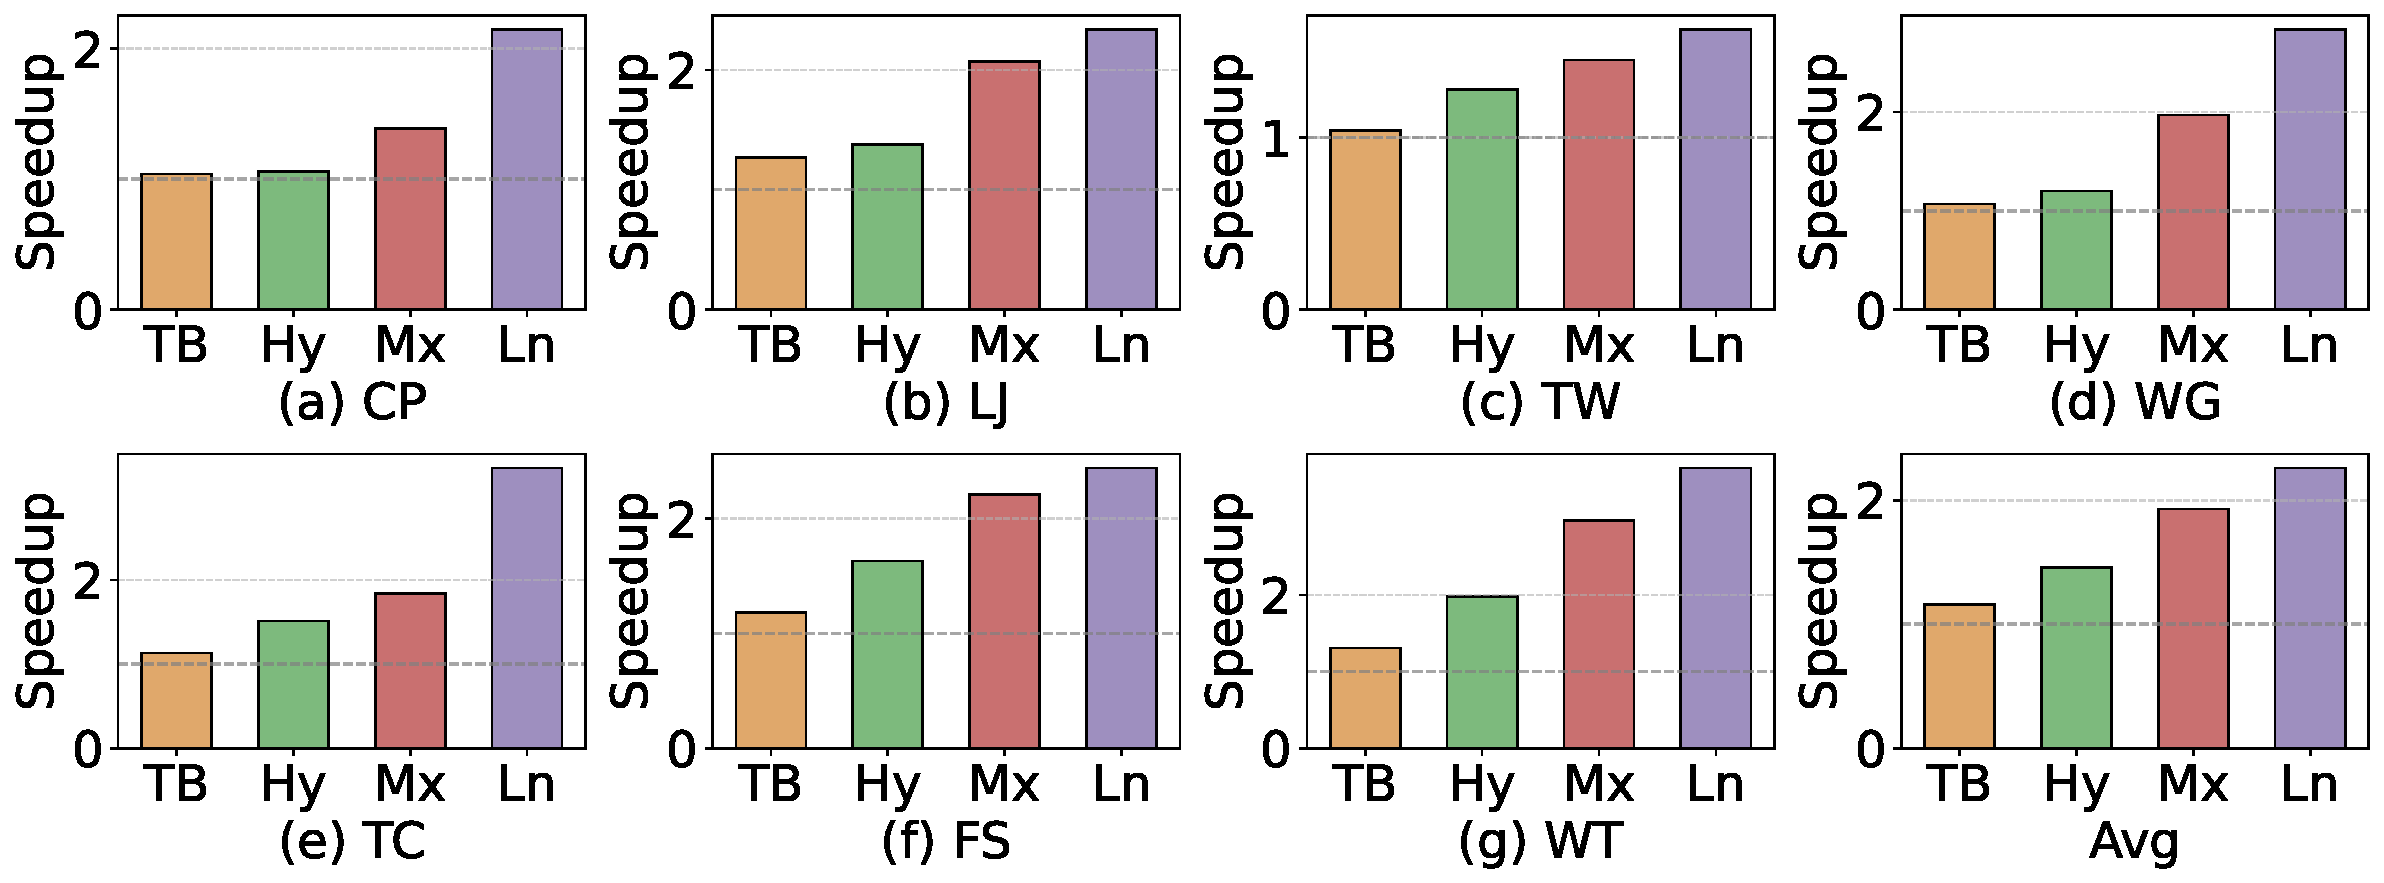
\includegraphics[width=1\linewidth]{figures/bfs_speedup_cropped.pdf}
%     \caption{Incremental speedups under progressive GIR optimizations for BFS, including TB, +Hy, +Mx, +Ln, respectively.}
%     % Each bar shows the cumulative speedup contributed by each technique (TB, +Hy, +Mx, +Ln) over a plain parallel BFS baseline.}
%     \label{fig:bfs_ablation}
% \end{figure}


% Figure~\ref{fig:bfs_ablation} reports the cumulative speedup at each stage for all seven graphs plus the average.
% Each technique contributes meaningfully, and the gains compound across the four stages.

% \textbf{TB} provides a moderate but consistent first-stage improvement.
% Graphs with large, dense frontiers (LJ, FS, WT) benefit the most, as switching from top-down to bottom-up traversal avoids redundant edge checks during peak frontier expansion.
% LJ reaches $1.27\times$ and WT reaches $1.31\times$ speedup over the plain BFS baseline at this stage.
% On TW, where the dominant SCC is extremely large, TB alone already reaches $1.04\times$, confirming that even a large frontier benefits modestly from direction switching.

% \textbf{+Hy} yields larger gains on graphs with a structurally dominant large block.
% Because the GIR hierarchy makes the largest BiCC block explicit, the hybrid strategy is applied selectively to that one block without disturbing the rest.
% WT jumps from $1.31\times$ to $1.98\times$ at this stage, and FS from $1.18\times$ to $1.63\times$, reflecting the high structural skewness of these social graphs where a single giant block dominates traversal cost.
% On CP and TC, which have a more uniform block-size distribution, the Hy gain is smaller ($1.0\times$ increment), since no single block is dominant enough to warrant a dedicated hybrid strategy.

% \textbf{+Mx} delivers the largest single-stage speedup increase across nearly all datasets.
% By dedicating threads to the largest block, this stage fully exposes the task parallelism that GIR's block decomposition provides.
% LJ reaches $2.07\times$ cumulative speedup, WG reaches $1.97\times$, and WT reaches $2.97\times$, all jumping by at least $0.7\times$ over the previous stage.
% TW's modest gain to $1.45\times$ reflects the limited number of independent blocks in its graph structure.

% \textbf{+Ln} provides the final speedup increment by replacing the parallel BFS kernel with a sequential linear scan for small blocks, eliminating synchronization overhead that dominates at small scales.
% TC benefits the most here, jumping from $1.84\times$ to $3.33\times$—the largest single-stage jump in the experiment—consistent with TC's exceptionally high count of small, loosely connected BiCC blocks.
% WT reaches its final $3.7\times$ speedup, the highest across all datasets, driven by both Hy and Ln acting on its highly skewed block-size distribution.

% Overall, the fully optimized configuration achieves speedups of $1.6\times$ (TW) to $3.7\times$ (WT), with an average of $2.3\times$ across all seven graphs (the Avg panel).
% The staircase pattern visible in every panel of Figure~\ref{fig:bfs_ablation} confirms that none of the four techniques is redundant: each addresses a distinct source of inefficiency exposed by the GIR hierarchy, and together they deliver substantial end-to-end acceleration.

\subsection{Scalability}
\begin{figure}[t]
    \centering
    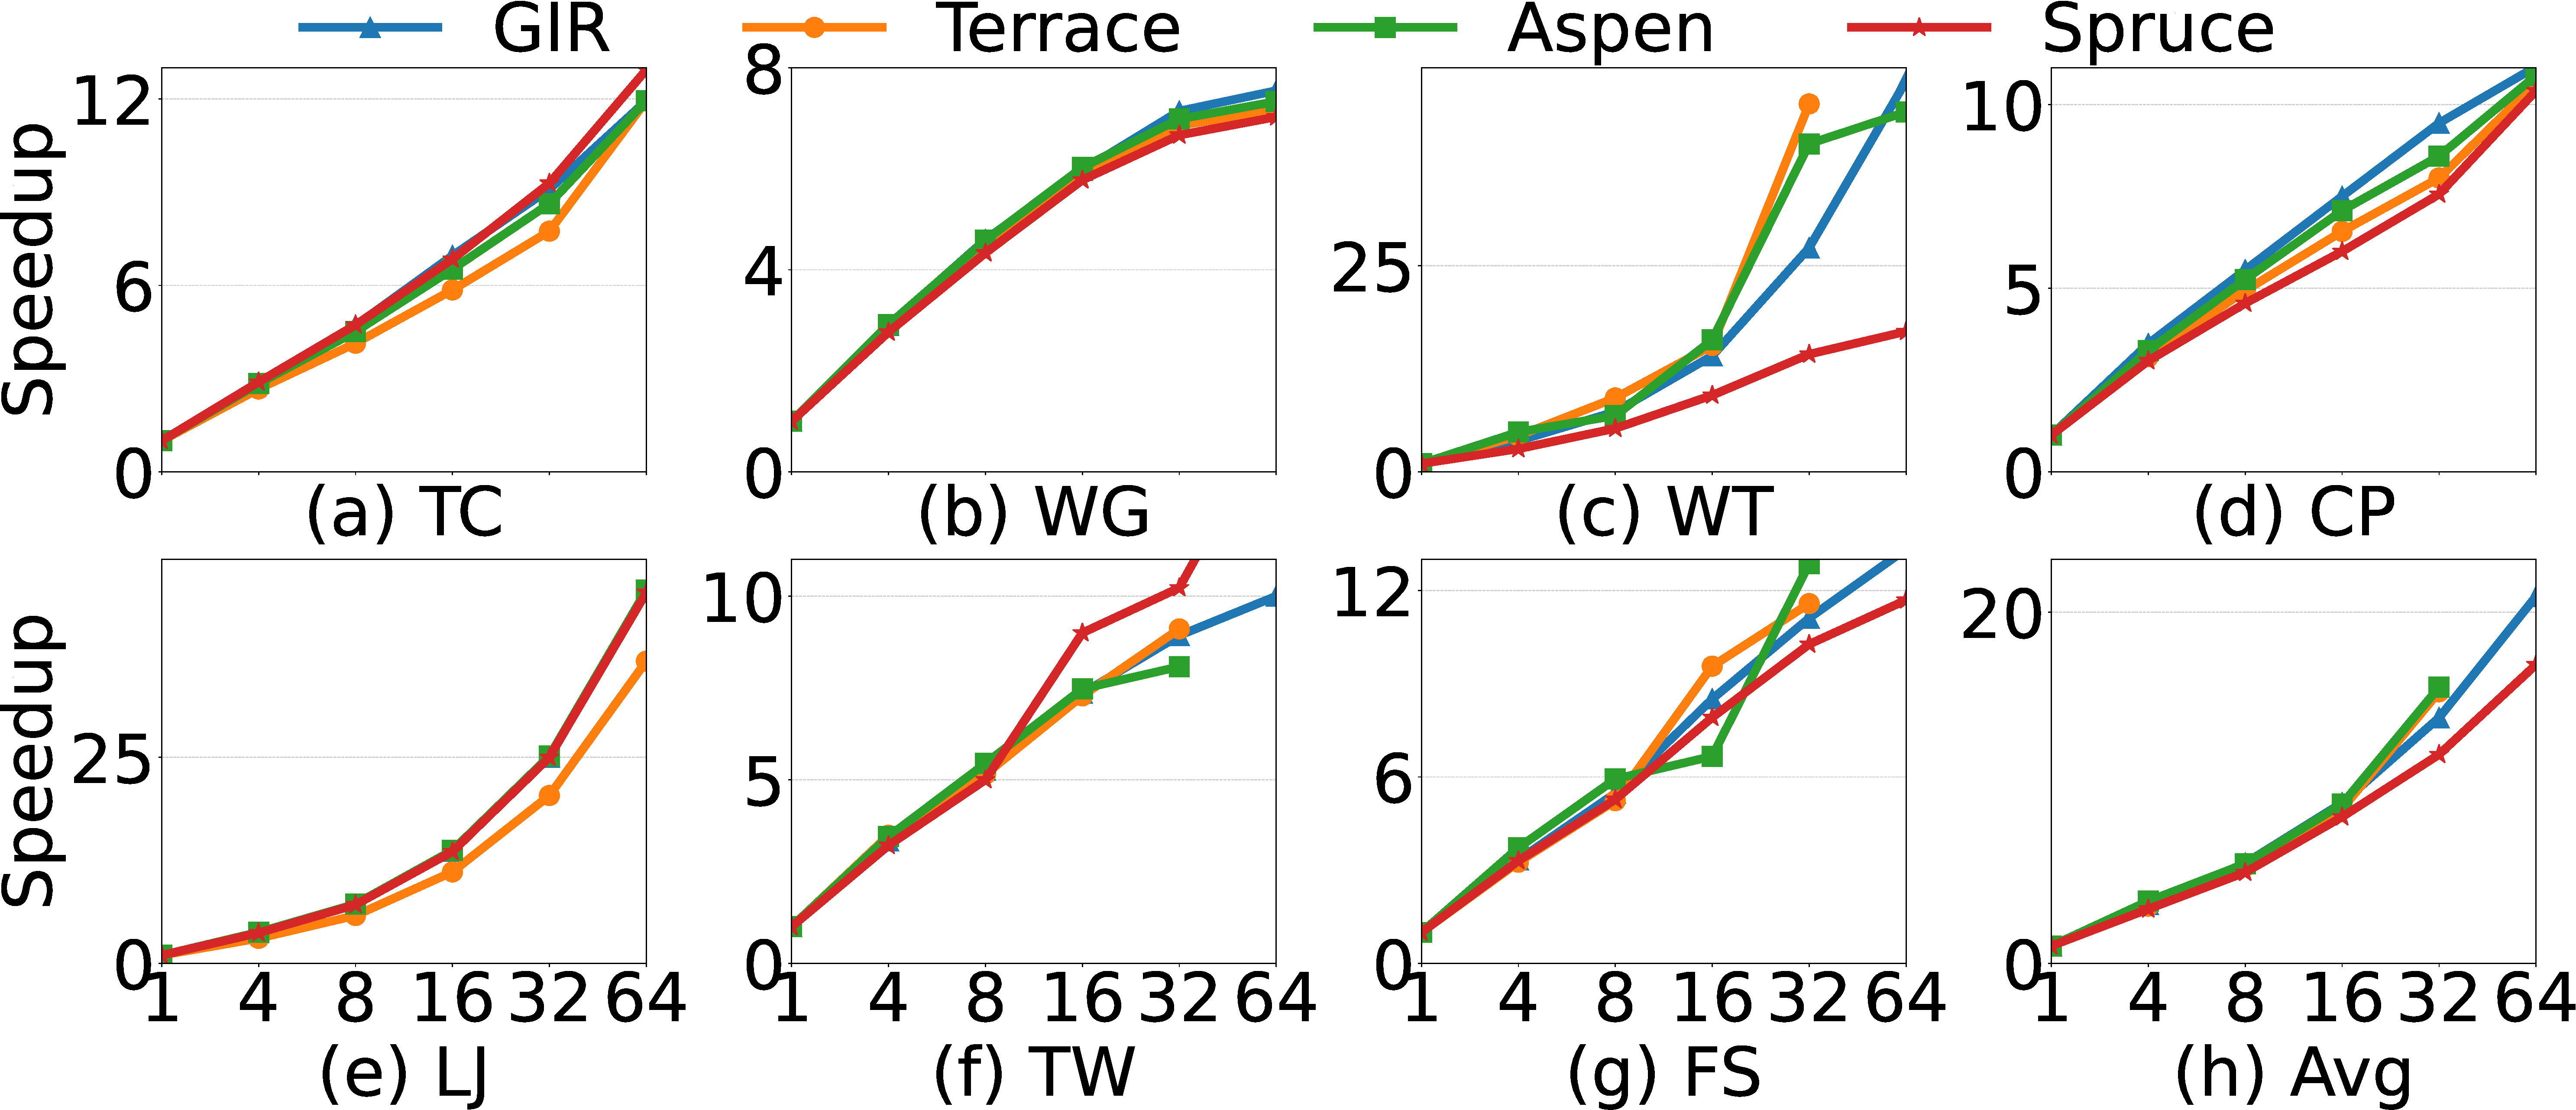
\includegraphics[width=1\linewidth]{figures/multiple_thread_speedup_all-crop.pdf}
    \caption{The BFS scalability against thread number. For TW and FS, Terrace and Aspen fail at 64 threads. For WT, Terrace fails at 64 threads.}
    \Description{Line charts of BFS speedup versus thread count (1 to 64) for GIR, Terrace, Aspen, and Spruce across seven datasets and their average.}
    % \caption{Multi-threaded BFS speedup of GIR, Terrace, Aspen, and Spruce on all seven datasets as the thread count increases from 1 to 64, where each system is normalized to its own single-threaded runtime.
    % For TW and FS, Terrace and Aspen fail at 64 threads; for WT, only Terrace fails at 64 threads.
    % Panel (h) shows the average speedup across all datasets; Terrace and Aspen averages are plotted only up to 32 threads.}
    \label{fig:mt_speedup}
\end{figure}


%We test the downstream graph query scalability by varying the number of threads from 1 to 64 across all seven datasets.
%Figure~\ref{fig:mt_speedup} shows the BFS speedup.
% normalized to GIR's single-threaded runtime.
%Note that all systems fail at 64 threads on TW and FS (the two largest graphs), and Terrace fails at 64 threads on WT. \YJ{Mismatch with the numbers reported in Table IV.}
% those curves are truncated at 32 threads accordingly.
%We make three observations.

We test the scalability of GIR by varying the number of threads from 1 to 64 across all seven datasets.
We take the BFS as a representative example.
Figure~\ref{fig:mt_speedup} shows the speedup of each method normalized to its own single-thread runtime.
Note that Terrace and Aspen fail at 64 threads on TW and FS, and Terrace fails at 64 threads on WT.
% their curves are truncated accordingly. 
% \YJ{Mismatch with the numbers reported in Table IV.}


% (i) GIR achieves the steepest scaling on graphs with many independent BiCC blocks.
% On WT (Figure~\ref{fig:mt_speedup}(c)), GIR reaches $47.4\times$ at 64 threads, ahead of Aspen ($43.6\times$) and Spruce ($17.0\times$).
% On LJ (Figure~\ref{fig:mt_speedup}(e)), all systems scale similarly well, with GIR reaching $45\times$ at 64 threads.
% On TC (Figure~\ref{fig:mt_speedup}(a)), GIR reaches $11.9\times$ at 64 threads, consistent with TC's exceptionally high count of small BiCC blocks.
% This steep scaling is driven by GIR's block-level task decomposition: each additional thread picks up independent block tasks with minimal inter-task coordination.

Particularly, we make three observations.
\textit{(i)} On average, GIR achieves $20.9\times$ speedups with 64 threads, way higher than Spruce's $17\times$.
Terrace and Aspen achieve $15.5\times$ and $15.7\times$ with 32 threads, respectively. They are omitted at 64 threads due to failures on TW and FS.


% The average scaling confirms GIR's strong aggregate scaling. 
% GIR's average speedup reaches $20.9\times$ from 1 to 64 threads, while Spruce reaches $17.0\times$. 
% Terrace and Aspen average reaches $15.5\times$ and $15.7\times$ from 1 to 32 threads, respectively.  
% they are omitted at 64 threads due to failures on TW and FS.

% The average scaling confirms GIR's strong aggregate scaling. 
% GIR's average speedup reaches $20.9\times$ from 1 to 64 threads, while Spruce reaches $17.0\times$. 
% Terrace and Aspen average reaches $15.5\times$ and $15.7\times$ from 1 to 32 threads, respectively.  
% they are omitted at 64 threads due to failures on TW and FS.

\textit{(ii)} GIR achieves the highest scaling on graphs with many independent BiCC blocks.
On WT, GIR achieves $47.4\times$ at 64 threads, higher than Aspen ($43.6\times$) and Spruce ($17\times$).
On LJ, all methods scale similarly well, with GIR reaching $45\times$ at 64 threads.
On TC, GIR achieves $11.9\times$ at 64 threads, mainly due to TC's exceptionally high count of small BiCC blocks.
% This steep scaling is driven by GIR's block-level task decomposition: each additional thread picks up independent block tasks with minimal inter-task coordination.

% (ii) GIR achieves the highest scalability on graphs with many independent BiCC blocks.
% On LJ and WT, GIR achieves $45\times$ and $47.4\times$ speedups at 64 threads, respectively, much higher than other baselines.
% On TC, which has an exceptionally high count of small BiCC blocks, GIR reaches $11.9\times$ at 64 threads with the largest gap over Spruce ($3\times$ from Table~\ref{tab:speedup_summary_alg}).
% This steep scaling is driven by GIR's block-level task decomposition: each additional thread picks up independent block tasks with minimal inter-task coordination.

\textit{(iii)} Scaling is more modest on graphs dominated by a few large SCCs.
On WG and CP, all methods scale similarly, with GIR reaching $7.5\times$ and $11\times$ at 64 threads.
On TW and FS, GIR achieves $8.9\times$ and $11.1\times$ at 32 threads before Terrace and Aspen fail to scale further.
% The limited block count in these graphs bounds the available task parallelism. 

% (i) GIR achieves the highest scalability on graphs with many independent BiCC blocks.
% On LJ and WT, GIR achieves $45\times$ and $47.4\times$ speedups at 64 threads, respectively, much higher than other baselines.
% On TC, which has an exceptionally high count of small BiCC blocks, GIR reaches $11.9\times$ at 64 threads with the largest gap over Spruce ($3\times$ from Table~\ref{tab:speedup_summary_alg}).
% This steep scaling is driven by GIR's block-level task decomposition: each additional thread picks up independent block tasks with minimal inter-task coordination.

%(i) GIR achieves the highest scalability on graphs with many independent BiCC blocks.
%On LJ and WT, GIR achieves $45\times$ and $47.4\times$ speedups at 64 threads, respectively, much higher than other baselines.
%On TC, which has an exceptionally high count of small BiCC blocks, GIR reaches $11.9\times$ at 64 threads with the largest gap over Spruce ($3\times$ from Table~\ref{tab:speedup_summary_alg}).
%This steep scaling is driven by GIR's block-level task decomposition: each additional thread picks up independent block tasks with minimal inter-task coordination.

%(ii) Scaling is more modest on graphs dominated by a few large SCCs.
%On WG and CP (Figure~\ref{fig:mt_speedup}(b)(d)), GIR reaches $7.3\times$ and $10.7\times$ at 64 threads.
%On TW and FS (Figure~\ref{fig:mt_speedup}(f)(g)), GIR reaches $8.9\times$ and $11.1\times$ at 32 threads before all systems fail to scale further.
%The limited block count in these graphs bounds the available task parallelism, but GIR still consistently leads all baselines at every thread count.

%(iii) The average panel (Figure~\ref{fig:mt_speedup}(h)) confirms that GIR's advantage compounds with thread count.
%GIR's average speedup reaches $24.5\times$ at 64 threads, while Spruce reaches $13.5\times$.
%Terrace and Aspen averages are omitted at 64 threads due to failures on multiple datasets.



% \subsection{Others?}
% \YJ{I would suggest we report as many expeirimental results as possible.}

%
%1. the distribution time of different size of blocks, 
%the total number of blocks are 1545753	
%biggest one is 824847	
%second one is 375651	
%third one is 686	
%fourth one 531	
%fifth one 348	
%...301	
%...98	
%the total number of BiCC with size 2 is 1100134	